\documentclass{article}
\usepackage[utf8]{inputenc}
\usepackage{pgfplots}
\usepackage[utf8]{inputenc}
\usepackage[shortlabels]{enumitem}
\usepackage{amsmath}
\usepackage{amssymb}
\usepackage{gensymb}
\usepackage{geometry}
\usepackage{listings}
\usepackage{xcolor}
\usepackage{pgfplots}
\usepackage{pgfplotstable}
\pgfplotsset{compat=1.7}
\usepackage{tikz}
\geometry{
 a4paper,
 total={170mm,257mm},
 left=20mm,
 top=20mm,
}
\title{Probability and Distribution Unit}
\author{Andy Yan}
\date{December 2022}

\begin{document}

\maketitle


\section{Set Notation}
\begin{center}
\def\arraystretch{1}
{\setlength{\tabcolsep}{3em}
\begin{tabular}{| c | c |} 
 \hline
   \textbf{Term} & \textbf{Symbol}\\ 
 \hline
Empty Set    & \(\emptyset\) \\
 \hline
Set of Natural Numbers	& \(\mathbb{N}\) \\
 \hline
Set of Integers	& \(\mathbb{Z}\) \\
 \hline
Set of Rational Numbers	& \(\mathbb{Q}\) \\
 \hline
Set of Real Numbers	& \(\mathbb{R}\) \\
 \hline
Set of Complex Numbers	& \(\mathbb{C}\) \\
 \hline
Is a member of	& \(\in\) \\
 \hline
Is not a member of	& \(\notin\) \\
 \hline
Owns	& \(\ni\) \\
 \hline
Is a proper subset of	& \(\subset\) \\
  \hline
Is a subset of	& \(\subseteq\) \\
  \hline
Is a proper superset of	& \(\supset\) \\
  \hline
Is a superset of	& \(\supseteq\) \\
  \hline
Set Union & \(\cup\) \\
    \hline
Set Intersection & \(\cap\) \\
    \hline
\end{tabular}}
\end{center}

\section{Probability and Distribution Notation}
\begin{center}
\def\arraystretch{1}
{\setlength{\tabcolsep}{3em}
\begin{tabular}{| c | c |} 
 \hline
   \textbf{Term} & \textbf{Symbol}\\ 
 \hline
Event A    & \(A\) \\
 \hline
Sample Space    & \(S\) \\
 \hline
Event A not occurring	& \(A'\) \\
 \hline
Event A or B occurring	& \(A \cup B\) \\
 \hline
Event A and B occurring	& \(A \cap B\) \\
 \hline
Event A occurring give Event B occurred	& \(A | B\) \\
 \hline
Odds & \(h : k\) \\
 \hline
 Number of Outcomes for Event A    & \(n(A)\) \\
 \hline
Probability of Event A occurring	& \(P(A)\) \\
 \hline
Probability of Success	& \(p\) \\
 \hline
Probability of Failure	& \(q\) \\
 \hline
Probability of Event X = x	& \(P(X = x)\) \\
  \hline
Expected Value of Event X	& \(E(X)\) \\
  \hline
\end{tabular}}
\end{center}

\section{Probability Rules}
\[P(A) = \frac{n(A)}{n(S)}\]
\[P(A') = 1 - P(A)\]
\[h : k, P(A) = \frac{h}{h+k}\]

\noindent
\begin{minipage}[t]{0.5\textwidth}
\begin{center}
    \textbf{Mutually Exclusive}
\end{center}
\[P(A \cup B) = P(A) + P(B) - P(A \cap B)\]
\end{minipage}% % leave no gap
\begin{minipage}[t]{0.5\textwidth}
\begin{center}
    \textbf{Non-Mutually Exclusive}
\end{center}
\[P(A \cup B) = P(A) + P(B)\]
\end{minipage}
\\\\
\begin{minipage}[t]{0.5\textwidth}
\begin{center}
    \textbf{Independent Events}
\end{center}
\[P(A \cap B) = P(A) \cdot P(B)\]
\[P(A' \cap B) = P(A') \cdot P(B) = (1 - P(A)) \cdot P(B)\]
\[P(A \cap B') = P(B') \cdot P(A) = (1 - P(B)) \cdot P(A)\]
\end{minipage}% % leave no gap
\begin{minipage}[t]{0.5\textwidth}
\begin{center}
    \textbf{Dependent Events}
\end{center}
\[P(A \cap B) = P(B) \cdot P(A|B) = P(A) \cdot P(B|A)\]
\[P(A|B) = \frac{P(A \cap B)}{P(B)} = \frac{P(A) \cdot P(B|A)}{P(B)}\]
\[P(B|A) = \frac{P(A \cap B)}{P(A)} = \frac{P(B) \cdot P(A|B)}{P(A)}\]
\end{minipage}
\begin{center}
    \textbf{Total Probability Formula}
\end{center}
\[P(A) = P(B) \cdot P(A|B) + P(B') \cdot P(A|B')\]
\[P(A) = P(A) \cdot P(B|A) + P(A') \cdot P(B|A')\]
\[P(A) = \Sigma P(B_i) \cdot P(A | B_i)\]

\section{Probability Distribution}
\textbf{Random Variable}\\
A random variable \((X)\) has a single value \((x)\) for each outcome in an experiment.
\[P(X), P(X=x_1),x_2,x_3,...,x_n\]
\begin{center}
    \textbf{Representations of Probability Distribution}\\
\end{center}
\begin{minipage}[t]{0.3333\textwidth}
\begin{center}
    \textbf{Numeral}
\end{center}
\begin{center}
\def\arraystretch{1}
{\setlength{\tabcolsep}{1em}
\begin{tabular}{| c | c |} 
 \hline
   \textbf{X} & \textbf{P(X)}\\ 
 \hline
1   & 1\slash 2 \\
 \hline
2    & 1\slash 3 \\
 \hline
3	& 1\slash 6 \\
 \hline
\end{tabular}}
\end{center}
\end{minipage}% % leave no gap
\begin{minipage}[t]{0.3333\textwidth}
\begin{center}
    \textbf{Graphical}
\end{center}
\begin{center}
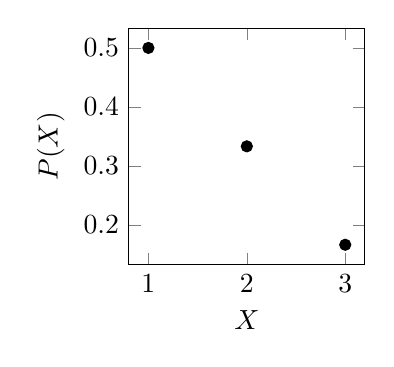
\begin{tikzpicture}
  \pgfplotsset{
      scale only axis,
  }
  \begin{axis}[
    xlabel=\(X\),
    ylabel=\(P(X)\),
    width=3cm,height=3cm,
  ]
    \addplot[only marks, mark=*]
    coordinates{ % plot 1 data set
      (1,0.5)
      (2,0.3333)
      (3,0.1666)
      % more points...
    }; \label{plot_one}
    % plot 1 legend entry
    \addlegendimage{/pgfplots/refstyle=plot_one}
  \end{axis}
\end{tikzpicture}
\end{center}
\end{minipage}
\begin{minipage}[t]{0.3333\textwidth}
\begin{center}
    \textbf{Algebraic}
\end{center}
\[P(X = a) = equation, a = 1, 2,...,n\]
\[P(X = a) = 5a^2, a = 1, 2, 3\]
\[P(X= 2) = 5 \cdot (2)^2 = 20\]
\end{minipage}
\textbf{Uniform Probability Distribution}\\
All outcomes are equally likely to occur for all values of X.
\[P(X) = \frac{1}{n(X)}\]
\textbf{Unitary Condition}\\
Holistic
\[P(X=x_1)+P(X=x_2)+...+P(X=x_n) = \sum_{k=1}^{n}P(X=x_k) = 1\]
\textbf{Expectation}
Expected outcome based on probability.
\[E(X) = x_1P(X=x_1)+x_1P(X=x_2)+...+x_nP(X=x_n) = \sum_{k=1}^{n}x_kP(X=x_k)\]

\section{Binomial Distribution}
\textbf{Conditions}\\
Success or failure. All trials are independent and the probability of each trial is the same. The random variable is the number of successes in a given number of trials.
\\
\noindent
\begin{minipage}[t]{0.5\textwidth}
\[P(X) = \binom{n}{x}p^xq^{n-x}\]
\begin{center}
\(n\) = \# of trials \\
\(x\) = \# of success 
\end{center}
\end{minipage}% % leave no gap
\begin{minipage}[t]{0.5\textwidth}
\break 
\begin{center}
\break
    \textbf{Expectation}
\end{center}
\[E(X) = n\cdot p\]
\end{minipage}
\section{Geometric Distribution}
Success or failure. The probability of success is the same for each observation and observations are all independent. The goal is to find the number of trials until the first success.\\
\noindent
\begin{minipage}[t]{0.5\textwidth}
\[P(X) = q^x p\]
\begin{center}
    \(x\) = \# of trials before success
\end{center}
\end{minipage}% % leave no gap
\begin{minipage}[t]{0.5\textwidth}
\begin{center}
    \textbf{Expectation}
\end{center}
\[E(X) = \displaystyle \sum_{k=0}^\infty k \cdot q^k p = \frac{q}{p} = \frac{1-p}{p}\]
\end{minipage}

\section{Hypergeometric Distribution}
Success or failure. Every trial is dependent, meaning the probability of success changes after each trial. The random variable is the number of successful trials in an experiment.\\
\noindent
\begin{minipage}[t]{0.5\textwidth}
\[P(X) = \frac{\binom{a}{x}\binom{n-a}{r-x}}{\binom{n}{r}}\]
\begin{center}
    \(x\) = given \# of successes\\
    \(r\) = \# of dependent trials\\
    \(a\) = \# successful outcomes\\
    \(n\) = \# total outcomes
\end{center}
\end{minipage}% % leave no gap
\begin{minipage}[t]{0.5\textwidth}
\begin{center}
    \textbf{Expectation}
\end{center}
\[E(X) = n\cdot \frac{a}{a+b} = \frac{r\cdot a}{n}\]
\end{minipage}


\end{document}
